\section{Définitions et propriétés}
\begin{df}
  Soit $(E, \mathcal T)$ un espace topologique. On dit que $E$ est séparable
  s'il existe un sous-ensemble $D$ de $E$ dénombrable tel que
  $\bar D = E$.
\end{df}

Un exemple d'espace séparable est $\mathbb R$ (avec sa topologie usuelle).
En effet, $\mathbb Q$ est un sous-ensemble dénombrable dense de $\mathbb R$.

\begin{prop}\label{sep:ind}
  Soient $(E, d)$ un espace métrique et $F\subseteq E$. Si $E$ est séparable,
  alors $F$ est séparable.
\end{prop}
\begin{proof}
  Soit $D = \{x_n \in E\mid {n\in\mathbb N}\}$ tel que $\bar D = E$.
  Pour tous $n$, $k$ naturels, $k\neq 0$, si
  $B\left(x_n, 1/k\right)\cap F$ est non
  vide, on choisit $y_{n, k}$ un élément de cette intersection. Posons
  $$L = \left\{y_{n, k} \in F\mid n, k\in\mathbb N, k \neq 0,
    B\left(x_n, \frac{1}{k}\right)\cap F\neq \varnothing\right\}$$
  et montrons que $\bar L = F$ (où on considère ici l'adhérence au sens
  de la topologie induite sur $F$).

  Soient $y\in F$ et $k$ un naturel non nul.
  Comme $\bar D = E$, il existe $n$ tel que $d(x_n, y) < 1/k$. Ceci implique
  que $B(x_n, 1/k)\cap F$ est non vide, et donc  $y_{n, k}$ est bien défini.
  On a, par l'inégalité triangulaire que $d(y, y_{n, k}) \leq d(y, x_n) +
  d(x_n, y_{n, k}) < 2/k$.

  Ceci montre que $\bar L = F$. Comme $L$ est au plus dénombrable,
  la preuve est terminée.
\end{proof}

\begin{prop}
  Soit $(E, \|.\|)$ un espace vectoriel normé. Les assertions suivantes sont
  équivalentes:
  \begin{enumerate}
  \item $E$ est séparable;
  \item $B(E) = \{x\in E\mid \|x\|\leq 1\}$ est séparable;
  \item $S(E) = \{x\in E\mid \|x\| =  1\}$ est séparable.
  \end{enumerate}
\end{prop}
\begin{proof}
  Au vu de la proposition \ref{sep:ind}, la première assertion implique
  la deuxième et la deuxième la troisième. On montre que la première
  est impliquée par la troisième.

  Soit $D = \{x_n \in S(E) | n\in\mathbb N\}$ tel que $\bar D = S(E)$.
  Posons $L = \{qx_n\mid q\in\mathbb Q^{>0}, n\in\mathbb N\}$. Alors $L$ est
  dense dans $E$ car pour tout vecteur $x\in E$,
  $$x = \|x\| \cdot \frac{x}{\|x\|}\in \left[0, +\infty \right[ \cdot S(E)
  = \mathrm{adh}_{\mathbb R}\mathbb Q^{>0}\cdot \mathrm{adh}_{E}D = \bar L.$$
  {L'argument sous-jacent à ces notations est que la multiplication
    scalaire $\mathbb R\times E\to E$ est continue et qu'en conséquence
    si $\lambda_n\to\lambda$ et $v_n\to v$ sont deux suites convergentes,
    respectivement une suite de réels et de vecteurs, alors la limite de
  la suite $\lambda_nv_n$ existe et vaut $\lambda v$}.
\end{proof}
\section{Exemples d'espaces séparables}
\textbf{Vous êtes invité à travailler ces exemples par vous-même avant de lire
les solutions.}
\begin{ex}
  L'espace de suites $(c_0, \|.\|_\infty)$ est séparable.
\end{ex}
\begin{proof}
  Soit $D = \{(q_0, \ldots, q_N, 0, \ldots)\mid
  N\in\mathbb N, q_j \in\mathbb Q\}$ l'ensemble des suites à coefficients
  rationnels ultimement nulles. Il s'agit d'un ensemble dénombrable
  (se plonge naturellement dans l'union dénombrable $\bigcup_{n}\IQ^n$).
  Montrons que $\bar D = c_0$.

  Soit $x = (x_n)_n\in c_0$.
  Soit $\epsilon > 0$. Il existe $N$ tel que tout $n\geq N$
  vérifie $|x_n|<\epsilon$. Pour $j = 0 \to N$, il existe $q_j\in \IQ$ tel
  que $|x_j-q_j|<\epsilon$ (car $\IQ$ est dense dans $\IR$). Dès lors,
  $(q_0, \ldots, q_N, \ldots)$ est élément de $D$ $\epsilon$-proche de $x$.

  Ceci termine la preuve.
\end{proof}

\begin{ex}
  Soit $p \in \left[1, +\infty\right[$.
  L'espace de suites $(\ell^p, \|.\|_p)$ est séparable.
\end{ex}
\begin{proof}
  Soit $D = \{(q_0, \ldots, q_N, 0, \ldots)\mid
  N\in\mathbb N, q_j \in\mathbb Q\}$ l'ensemble des suites à coefficients
  rationnels ultimement nulles. Il s'agit d'un ensemble dénombrable.

  Soient $x = (x_n)_n\in \ell ^p$ et $\epsilon >0$. Il existe $N$ tel que
  pour tout $n \geq N$,
  $$\sum_{k=n}^{+\infty}|x_k|^p < \epsilon.$$
  Pour $j = 0 \to N$, il existe $q_j$ rationnel tel que
  $|x_j-q_j|^p<\epsilon/N$. Posons $u=(q_0, \ldots, q_N, 0, \ldots)\in D$, alors
  $\|u-x\|^p_p<2\varepsilon$.

  Ceci termine la preuve.
\end{proof}

\begin{rem}
  Dans les deux exemples précédents, on a considéré $c_0$ et $\ell^p$
  comme $\IR$-espaces vectoriels normés. Si on considère leur analogue
  complexe, il est nécessaire de considérer l'ensemble des suites à
  coefficients dans $\IQ(i)$ (ou un autre sous-ensemble dénombrable dense
  de $\IC$) ultimement nulles, plutôt que $\IQ$.
\end{rem}

\begin{ex}
  $\mathcal C([0, 1]; \IR)$ est séparable.
\end{ex}
\begin{proof}
  Le théorème d'approximation de Weierstrass assure que l'espace des polynômes
  est dense dans $\mathcal C([0, 1]; \IR)$. Il suffit donc de montrer qu'il
  existe un sous-ensemble de l'espace des polynômes dénombrable dont l'adhérence
  contient l'espace des polynômes\footnote{Rappel: Soient $(X, \mathcal T)$ un
    espace topologique, $D$ dense dans $X$ et $E\subseteq D$ tel
    que $D\subseteq \bar E$. Par monotonicité de l'adhérence, on a
    $X = \bar D \subseteq \bar{\bar E} =\bar E$, donc $E$ est également dense.}.

  Il suffit de considérer l'ensemble des polynômes à coefficients
  rationnels. Il est bien dense dans l'ensemble des polynômes (car $\IQ$
  est dense dans $\IR$).
\end{proof}
\section{Exemples d'espaces non-séparables}
\textbf{Rappel}: $|\mathcal P (\mathbb N)| = |\mathbb R| = 2^{\aleph_0}$.

Avant de présenter des exemples, on introduit un résultat utile pour montrer
qu'un espace métrique n'est pas séparable.

\begin{prop}
  Soit $(E, d)$ un espace métrique. S'il existe $B\subseteq E$ non dénombrable
  tel que tous $b_1$, $b_2\in B$ distincts on a $d(b_1, b_2)\geq 1$ alors
  tout sous-ensemble $A$ dense de $E$ est non dénombrable.
\end{prop}
\begin{proof}
  Soient $b_1$, $b_2$ deux éléments de $B$. \`A l'aide de l'inégalité
  triangulaire, on obtient que $B(b_1, 1/4)\cap B(b_2, 1/4)=\varnothing$
  (sinon $b_1$ et $b_2$ sont $1/2$-proches).

  Soit $A$ un sous-ensemble dense de $E$. Alors $A$ intersecte chacune des
  boules $B(b, 1/4)$, $b\in B$. Comme elles sont disjointes et que
  $B$ est non dénombrable, cela assure que $A$ est non dénombrable.
\end{proof}

\begin{cor}\label{sep:neg}
  Soit $(E, d)$ un espace métrique. S'il existe $B\subseteq E$ non dénombrable
  tel que tous $b_1$, $b_2\in B$ distincts on a $d(b_1, b_2)\geq 1$ alors
  $E$ n'est pas séparable.
\end{cor}

\begin{ex}
  L'espace de suites $\ell^\infty$ n'est pas séparable.
\end{ex}
\begin{proof}
  On applique le corollaire \ref{sep:neg}. On prend le sous-ensemble
  de $\ell^\infty$ suivant:
  $$B = \{x = (x_n)_n\in\ell^\infty\mid
  \forall n, x_n= \ind_A(n), A\subseteq \IN\}.$$
  L'ensemble $B$ est bien non dénombrable (on peut y plonger les parties
  de $\IN$) et deux éléments distincts seront distants de 1; étant données
  deux parties différentes de $\IN$, il existe un naturel dans une partie
  et pas l'autre, et les suites associées vaudront respectivement 0 et 1
  en la composante correspondante, ce qui implique l'affirmation.
\end{proof}

\begin{ex}
  $(\mathcal C([0, 1]; \IR))^*$ n'est pas séparable.
\end{ex}
\begin{proof}
  Soit pour $t\in [0, 1]$ la forme linéaire $\ev_{t}: C([0, 1]; \IR) \to \IR:
  f\mapsto f(t)$. Cette forme est continue car pour $f\in C([0, 1]; \IR)$,
  $|\ev_t(f)|\leq \|f\|_\infty$.

  On montre que la famille $(\ev_t)_{t\in[0, 1]}$ satisfait les hypothèses
  du corollaire \ref{sep:neg}. Il s'agit bien d'une famille non dénombrable
  d'éléments de $(\mathcal C([0, 1]; \IR))^*$. Considérons maintenant $t$, $s
  \in[0, 1]$, $t\neq s$. Pour montrer que $\ev_t$ et $\ev_s$ vérifient
  $\|\ev_t-\ev_s\|\geq 1$, il suffit de prendre une fonction de norme au
  plus $1$ similaire à celle illustrée à la figure \ref{sepa:ill}.
  % Figure pour illustrer les fonctions à choisir pour montrer que le
% dual de C[0, 1] n'est pas séparable.
\begin{figure}[!h]
  \begin{center}
    \caption{Fonction $f$ illustrant $\|\ev_t-\ev_s\|\geq 1$}%
    \label{sepa:ill}
    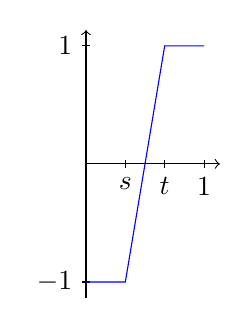
\begin{tikzpicture}[scale=0.5]
      \draw [->] (0, -3.4) -- (0, 3.4);
      \draw [->] (0, 0) -- (3.4, 0);
      \draw (1, 0.1) -- (1, -0.1) node [below] {$s$};
      \draw (2, 0.1) -- (2, -0.1) node [below] {$t$};
      \draw (3, 0.1) -- (3, -0.1) node [below] {$1$};
      \draw (0.1, 3) -- (-0.1, 3) node [left] {$1$};
      \draw (0.1, -3) -- (-0.1, -3) node [left] {$-1$};
      \draw [blue] (0, -3) -- (1 , -3) -- (2, 3) -- (3, 3);
    \end{tikzpicture}
\end{center}
\end{figure}


%%% Local Variables:
%%% mode: latex
%%% TeX-master: "../analyse3"
%%% End:

\end{proof}

\begin{ex}
  $\mathcal L(\ell^2)$ n'est pas séparable.
\end{ex}
\begin{proof}
  Notons chaque élément de $\ell^2$ comme suit:
  $$(x_n)_n = \sum_{n=0}^\infty x_n e_n.$$

  Soit $A\subseteq \IN$, on pose
  $$T_A: \ell^2 \to\ell^2: \sum_{n=0}^\infty x_n e_n \mapsto
  \sum_{n\in A} x_n e_n.$$

  On vérifie facilement que $T_A$ est bien définie, linéaire et continue
  (on a $\|T_A\|= 1$ si $A$ est non vide, sinon $T_A$ est l'application nulle).
  L'ensemble $B = \{T_A\mid A\subseteq \IN\}$ vérifie les hypothèses du
  corollaire  \ref{sep:neg}; il s'agit bien d'un ensemble non dénombrable
  de $\mathcal L(\ell^2)$, et étant donnés $A, A'\subseteq \IN$, $A\neq A'$,
  alors il existe (sans perte de généralité, quitte à échanger $A$ et $A'$)
  $n\in A\setminus A'$, d'où $T_A(e_n) = 1$ et $T_{A'}(e_n) = 0$ ce qui
  implique  $\|T_A - T_{A'}\|\geq 1$.
\end{proof}
%%% Local Variables:
%%% mode: latex
%%% TeX-master: "../analyse3"
%%% End:
